\documentclass[letterpaper]{article} % DO NOT CHANGE THIS
\usepackage[submission]{aaai2027}  % DO NOT CHANGE THIS (anonymous, double-blind)
% The serif, sans-serif, and monospaced fonts are loaded automatically by
% aaai2027.sty (newtxtext, helvet, courier). DO NOT add any font package.
\usepackage[hyphens]{url}  % DO NOT CHANGE THIS
\usepackage{graphicx} % DO NOT CHANGE THIS
\urlstyle{rm} % DO NOT CHANGE THIS
\def\UrlFont{\rm}  % DO NOT CHANGE THIS
\usepackage{natbib}  % DO NOT CHANGE THIS AND DO NOT ADD ANY OPTIONS TO IT
\usepackage{caption} % DO NOT CHANGE THIS AND DO NOT ADD ANY OPTIONS TO IT
\frenchspacing  % DO NOT CHANGE THIS
% common/preamble.tex: shared by every FactorJEPA workshop draft (paper-variants skill). Edit once here;
% a sentence that must differ for one venue goes behind a venue switch in common/, never into a second copy.
\usepackage{booktabs}
\usepackage{amsmath}
\usepackage{amssymb}
\graphicspath{{../common/figs/}}
% common/numbers.tex: every measured number that a venue part (title, abstract, introduction, venue discussion)
% states. Venue files never type a measured number; build_all.py refuses one. Shared sections in common/ state
% their numbers once, so a change there reaches every draft.
% Sources:
%   dataset counts: dataset card src/hf_denseworld_115k/README.md and sources.json (714 videos, 22 cities);
%   separations at 1B, 115k clips: Figure 3 (common/figs/forest_115k_col.png, src/m13_eval_plot.py on outputs/full);
%   ladder: common/results/*.json (src/utils/paired_ladder.py, outputs/workshop/attribution_10k).
\newcommand{\nClips}{115,687}
\newcommand{\nHours}{276}
\newcommand{\nVideos}{714}
\newcommand{\nCities}{22}
\newcommand{\nAnnotated}{86,831}
\newcommand{\nSepLo}{13.9}
\newcommand{\nSepHi}{43.3}
\newcommand{\nFutPct}{2.7\%}
\newcommand{\nMaskPct}{19\%}
\newcommand{\nRawFutTwoB}{0.036}
\newcommand{\nRawFutOneB}{0.020}
\newcommand{\nLadderMaskTwoB}{6.0\%}  % Ours vs RAW Mask-ratio slope, exact 5.97% (common/results, means.maskratio)
\newcommand{\nLadderMaskOneB}{2.4\%}  % exact 2.41%; was rounded to 2% before the Nov 27 judges' round
\newcommand{\nTestVideos}{127}
\newcommand{\nHeldoutClips}{1,702}  % video-disjoint check, 1B 10k models (common/results/heldout_video_1B10k_paired.json)
\newcommand{\nHeldoutVideos}{136}   % source videos with no training or validation clip
  % venue parts state measured numbers only through these macros
\hyphenation{DENSEWORLD}
% Double-blind: no build date, time zone or TeX banner in the PDF metadata.
\pdfinfoomitdate=1
\pdftrailerid{}
\pdfsuppressptexinfo=-1
% venue switches (set in each venue folder's venue.tex, read after this file)
\newif\ifanon          % double-blind venue: no names, no identifying links
\newif\ifvenueCog      % Cog2Soc bridge (collective human behaviour)
\newif\ifvenueData     % Data2AgentEx bridge (domain data to agent experience)
\newif\ifvenueCausal   % Continual Causality bridge, novel-work track
\newif\ifvenueAgms     % Human-Centric AgMS workshop (W4, mobility agents)
% common/disclosure.tex: anonymous concurrent-submission note (owner pick Fri Nov 27 2026 ~6:40 AM PST).
% All four venues review double-blind and their OpenReview forms have no field for other submissions, so the
% note sits in the PDF: it names the other three AAAI-27 venues, never the authors or the arXiv number.
% Each venue draft uses it once, as \footnote{\disclosure} at the end of its first introduction paragraph.
% Every branch ends with "<sentence>. \fi%": the space before \fi survives, the line end after it does not.
\newcommand{\disclosure}{Concurrently under review, all non-archival: %
\ifvenueCog the AAAI-27 Data2AgentEx and Continual Causality bridges and the Human-Centric AgMS workshop. \fi%
\ifvenueData the AAAI-27 Cog2Soc and Continual Causality bridges and the Human-Centric AgMS workshop. \fi%
\ifvenueCausal the AAAI-27 Cog2Soc and Data2AgentEx bridges and the Human-Centric AgMS workshop. \fi%
\ifvenueAgms the AAAI-27 Cog2Soc, Data2AgentEx, and Continual Causality bridges. \fi%
An earlier version is a non-archival AAAI-27 student abstract and a public preprint.}
  % \disclosure: concurrent-submission footnote text, switched per venue

% venue switches for Human-Centric AgMS (AAAI-27 Workshop W4, "Human-Centric Agentic Mobility Services"): double-blind
% (OpenReview submission invitation hides authors from reviewers, read 2026-11-27), AAAI-27 author kit, at most 4 pages
% excluding references, non-archival, concurrent submissions allowed. Call: agentic-mobility-workshop.github.io/cfp.html.
% pages: 4
% due: Fri Dec 25 2026 8:59 PM PST
\venueAgmstrue
\anontrue

\pdfinfo{
/TemplateVersion (2027.1)
}

\setcounter{secnumdepth}{2}

% VENUE PARTS ONLY (paper-variants skill): title, abstract, introduction and the venue discussion section live here;
% the dataset, method, evaluation and scope sections, figures, tables, numbers and bibliography live once in ../common/.
% AAAI-27 workshop "Human-Centric Agentic Mobility Services" (Montreal, Feb 22 or 23, 2027).
% Rules (CFP, agentic-mobility-workshop.github.io/cfp.html): research / position / benchmark / dataset / demo papers,
% at most 4 pages EXCLUDING references, AAAI-27 author kit, double-blind on OpenReview (Human-Centric_AgMS),
% non-archival, concurrently submitted work allowed, in-person presentation. Due Fri Dec 25 2026 8:59 PM PST
% (OpenReview); results Sat Jan 2 2027. Kit: appendices count toward the page limit; no supplement.
% 2026-11-27 (owner picks): moved onto ../common/, so this draft now carries the Cog2Soc v3 fixes: the method is the
% 3-stage layout, agent, interaction clip curriculum that src/m09c1_surgery_encoder.py trains (the earlier text described
% a factorized predictor that was never implemented), Table 2 attribution ladder, release paragraph, one-column Figure 2,
% scope section. Own venue title; anonymous concurrent-submission footnote (common/disclosure.tex).

\title{Can a World Model of Traffic Scenes Predict Crowded South Asian Streets?}  % owner pick Fri Nov 27 2026 ~6:30 AM PST: one title per venue (the arXiv and student-abstract title stays 'FactorJEPA on DENSEWORLD-115k: ...')

\author{Anonymous Submission}
\affiliations{}

\begin{document}

\maketitle

\begin{abstract}
A mobility agent that drives, walks, or dispatches in a crowded city has to anticipate what pedestrians, two-wheelers, auto-rickshaws, carts, and animals will do next, often while they are partly hidden. Video world models such as V-JEPA 2.1 forecast the future in embedding space, but world models of traffic scenes are trained and evaluated mostly on lower-density, lane-structured traffic. We build DENSEWORLD-115k, \nClips{} clips (\nHours{} hours) cut from \nVideos{} public YouTube videos of \nCities{} Indian cities, released as reconstructible metadata, and FactorJEPA, a curriculum that adapts V-JEPA 2.1 first on clips of the street layout, then on the road users, then on their interactions. Compared with seven adaptation methods under identical clips and budgets, one fixed FactorJEPA configuration predicts masked and future content better at both 2B and 1B scale, and after full 115k-clip training it separates from the stronger of the two rivals trained at that scale on all four diagnostics of predictive structure, by \nSepLo{} to \nSepHi{} widths of the paired 95\% confidence interval. An ablation on raw clips shows that the staged adaptation carries most of this gain, while the layout, agent, and interaction clips make prediction more robust when more of the scene is hidden. Competing methods still lead on temporal coherence. We discuss what such a traffic-scene world model can and cannot yet offer mobility agents.
\end{abstract}

\begin{links}
    \link{Dataset}{https://huggingface.co/datasets/anonymousML123/denseworld-115k}
\end{links}


\section{Introduction}

Agentic mobility services, from driver assistants to delivery robots and fleet dispatchers, act among road users whose next move they must predict. World models of traffic scenes supply that prediction. Joint Embedding Predictive Architectures (JEPA) such as V-JEPA 2.1 \cite{murlabadia2026vjepa21} learn it without labels by predicting masked or future video content as embeddings rather than pixels. A traffic scene has layers that matter differently to such an agent: the road layout, the individual road users, and the interactions between them, and they are hardest to predict where all three are tightly coupled.\footnote{\disclosure}

South Asian streets are such a regime. Road edges are negotiated rather than painted, pedestrians and vehicles of very different speeds share one right of way, clutter keeps road users partly hidden, and who goes first is settled by local norms more than by lane rules. Driving benchmarks such as BDD100K \cite{yu2020bdd100k} and nuScenes \cite{caesar2020nuscenes} sample this regime rarely. We adapt V-JEPA 2.1 to it layer by layer and contribute:
\begin{itemize}
    \item \textbf{DENSEWORLD-115k}, a \nHours{}-hour drive-through, walk-through, and aerial video corpus of \nCities{} Indian cities, released as reconstructible metadata.
    \item \textbf{FactorJEPA}, a three-stage curriculum that adapts V-JEPA 2.1 on layout, agent, and interaction clips derived automatically from the video, with no extra inputs at inference.
    \item A controlled comparison with seven adaptation methods at two model and two data scales on all 13 diagnostics, wins and losses alike, and an ablation that separates the staged adaptation from the curriculum's clips.
\end{itemize}

\begin{figure*}[t]
\centering
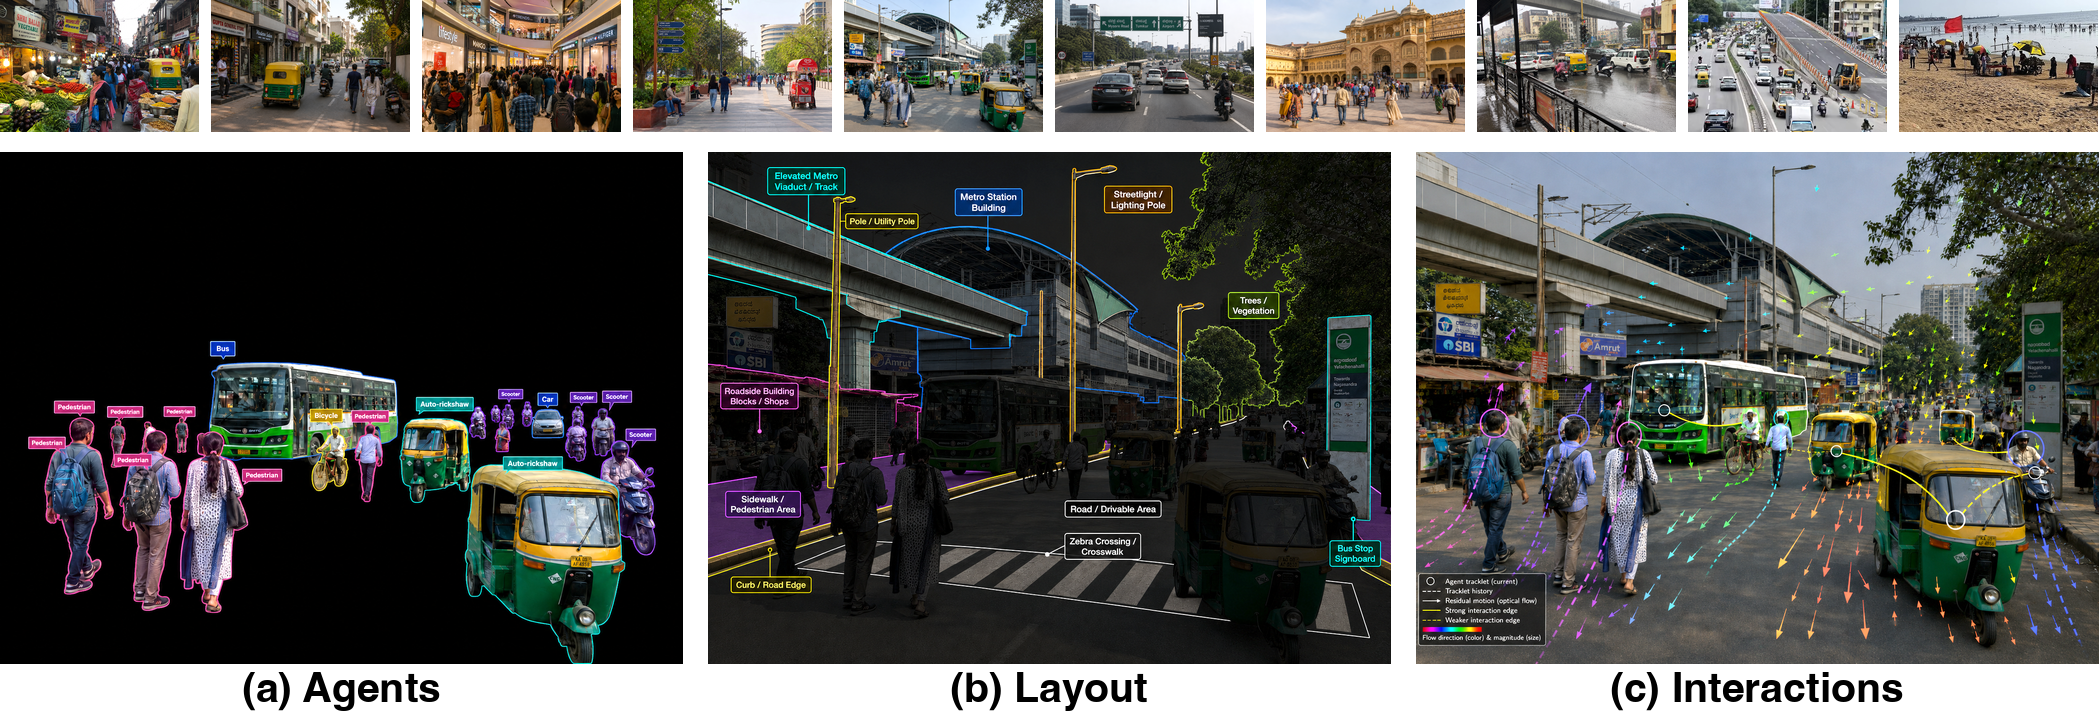
\includegraphics[width=\textwidth]{denseworld_teaser.png}
\caption{Generated illustrations, not dataset frames. Top: the ten DENSEWORLD-115k scene types (market, residential, commercial, promenade, transit, highway, heritage, junction, flyover, beach). Bottom: the three clip types FactorJEPA trains on: (a) road users with the background suppressed, (b) the layout with road users suppressed, and (c) interactions between tracked road users (circles: road users; arrows: motion; solid or dashed edges: stronger or weaker coupling).}
\label{fig:teaser}
\end{figure*}


\section{DENSEWORLD-115k}

DENSEWORLD-115k records everyday street behaviour in 22 Tier-1 and Tier-2 Indian cities: 115,687 clips of 4 to 14 seconds (median 9.3; 276 hours; Figure~\ref{fig:teaser}, top), cut with scene and shot-boundary detection from 714 public long-form YouTube videos (480p). It covers drive-through, walk-through, and aerial viewpoints across markets, residential lanes, transit corridors, junctions, flyovers, heritage sites, and beaches, at different times of day and in different weather. For 86,831 clips an automatic pipeline finds the road users: Grounding DINO \cite{liu2024groundingdino} detects them on anchor frames, SAM~3 \cite{carion2025sam3} tracks their masks through the clip, and pairs of road users that are close and move relative to each other are marked as candidate interactions.

\begin{figure}[t]
\centering
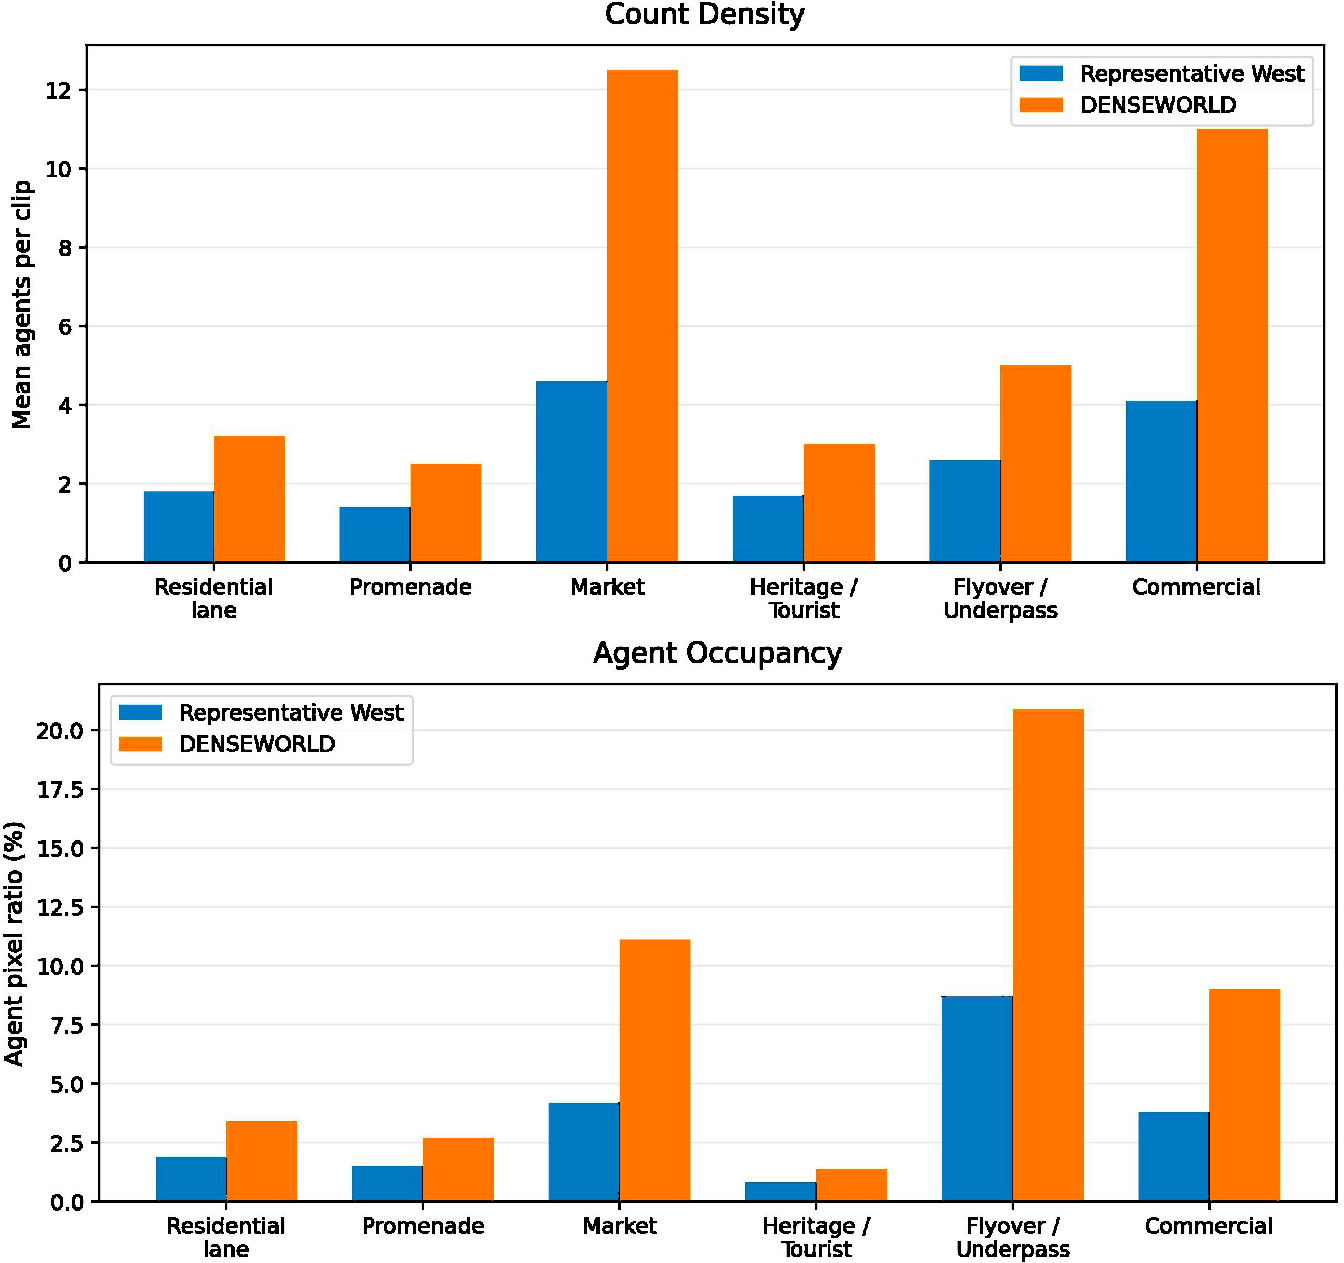
\includegraphics[width=\columnwidth]{denseworld_vs_west_density_bold.pdf}
\caption{Mean agents per clip (top) and share of pixels covered by agents (bottom) for DENSEWORLD and a Western reference drawn from BDD100K and nuScenes, per scene type.}
\label{fig:density}
\end{figure}

Against a reference set of BDD100K and nuScenes clips grouped by the same scene types, DENSEWORLD has more agents per clip and a larger share of pixels covered by agents on each of the six types compared (Figure~\ref{fig:density}). Agent count and pixel occupancy establish this density shift on all six matched types and motivate occlusion and interaction pressure as the next axes to measure. A \ifvenueCog behaviour\else world\fi{} model calibrated on the Western reference therefore meets a shifted distribution here, the setting in which we evaluate adaptation.

\paragraph{Release and responsible use.} Respecting the creators' copyright, the release ships the source list, the clip manifest with timestamps, and a deterministic script that rebuilds every clip from YouTube, rather than the videos, under a CC BY 4.0 licence for the metadata. The metadata release depends on creator-hosted videos: a video its creator removes can no longer be rebuilt, and rights holders can ask on the dataset page for a source to be removed. The corpus is meant for research on aggregate street behaviour, not on individuals, because the people filmed did not consent individually.


\section{FactorJEPA}

FactorJEPA keeps V-JEPA 2.1's encoder, predictor, masking policy, and prediction objective, and changes what the model is trained on and which blocks it updates. From a checkpoint already adapted to the corpus by plain continued pretraining, it trains in three stages on clips built from the automatic masks (Figure~\ref{fig:teaser}, bottom): layout clips in which every detected road user is blurred; then agent clips in which the background is suppressed, mixed 70/30 with layout clips; then interaction clips, cropped around pairs of interacting road users, mixed 70/15/15 with the other two. Half of the training samples are raw clips, which keeps the model anchored to ordinary video. The first stage unfreezes the first 4 of the encoder's 48 blocks and the later stages the first 8, following surgical fine-tuning \cite{lee2023surgical}; the predictor trains throughout against a frozen teacher, selective projection decay \cite{tian2024spd} keeps the weights near their starting point, and the fixed configuration splits its epochs 30/25/45 across the stages. At inference FactorJEPA is an ordinary V-JEPA model: no detector, tracker, or mask is needed. Unlike SlotFormer's object-centric slots \cite{wu2023slotformer} and DriveWorld's split of static scene from dynamics \cite{min2024driveworld}, FactorJEPA keeps one predictor and builds the layout, agent, and interaction structure into what it trains on.


\section{Evaluation}

\paragraph{Protocol.}
We adapt V-JEPA 2.1 at 2B and 1B parameters on a stratified 10k-clip set, and the 1B model also on the full corpus. FactorJEPA is compared with the frozen backbone, full fine-tuning, linear probing then fine-tuning \cite{kumar2022finetuning}, continual self-supervised learning (plain continued pretraining with the V-JEPA objective), LoRA \cite{hu2022lora}, DoRA \cite{liu2024dora}, and Auto-RGN \cite{lee2023surgical}, all under identical clips, masking, optimization steps, and splits. Every other trained method starts from that continued-pretraining checkpoint, which saw the training clips only, so no method sees a validation or test clip; the frozen backbone is V-JEPA 2.1 as released. Test clips are held out at the clip level (1,825 in the 10k regime, 23,106 in the full regime), so a source video can contribute clips to both training and test (Section~\ref{sec:scope}). Every margin is a paired 95\% BCa bootstrap interval over test clips.

\paragraph{Diagnostics of predictive structure.}
\emph{Future-frame L1}: error between predicted and target-encoder embeddings on the token blocks hidden by V-JEPA's mask generator. \emph{Forward L1}: the same error when the second half of a clip is predicted from its first half. \emph{Mask-ratio slope}: growth of that error as the hidden fraction rises from 0.3 to 0.9. \emph{Motion cosine}: how much closer a test clip's mean-pooled embedding lies to clips of its own motion class than to clips of other classes, with no training; the 16 motion classes come from optical flow (speed quartile by dominant direction). Nine further diagnostics probe temporal coherence and semantics (Table~\ref{tab:headline}). Small heads trained on the frozen embedding measure temporal order (pick the true frame order among permutations), pace (recognise the playback speed), action top-1 (an attentive probe for the motion class), and arrow-of-time (forward versus reversed playback). TCC $\tau$ and TCC cycle error test, with no training, whether matching moments of two clips align. With the predictor fed its own outputs, exposure bias is the error gap to feeding it the true frames, rollout drift is the error growth per step, and L1-vs-$\Delta t$ is the error growth with the prediction horizon.

\begin{table}[t]
\centering
\small
\setlength{\tabcolsep}{2pt}
\begin{tabular}{lrrrrrr}
\toprule
 & \multicolumn{2}{c}{2B$\cdot$10k} & \multicolumn{2}{c}{1B$\cdot$10k} & \multicolumn{2}{c}{1B$\cdot$115k} \\
\cmidrule(lr){2-3}\cmidrule(lr){4-5}\cmidrule(lr){6-7}
Diagnostic & Ours & Rival & Ours & Rival & Ours & Rival \\
\midrule
future-frame L1 ($\downarrow$) & \textbf{0.496} & 0.504\textsuperscript{L} & \textbf{0.590} & 0.596\textsuperscript{L} & \textbf{0.573} & 0.589\textsuperscript{L} \\
forward L1 ($\downarrow$) & \textbf{0.529} & 0.533\textsuperscript{L} & \textbf{0.614} & 0.617\textsuperscript{L} & \textbf{0.597} & 0.607\textsuperscript{L} \\
mask-ratio slope ($\downarrow$) & \textbf{0.053} & 0.054\textsuperscript{L} & \textbf{0.052} & 0.053\textsuperscript{D} & \textbf{0.047} & 0.058\textsuperscript{L} \\
motion-cos ($\uparrow$) & 0.116 & \textbf{0.244}\textsuperscript{F} & 0.048 & \textbf{0.090}\textsuperscript{F} & \textbf{0.097} & 0.078\textsuperscript{L} \\
\midrule
temporal-order ($\uparrow$) & 0.944 & \textbf{0.947}\textsuperscript{Z} & 0.925 & \textbf{0.927}\textsuperscript{C} & \textbf{0.918} & 0.915\textsuperscript{Z} \\
pace ($\uparrow$) & 0.719 & \textbf{0.724}\textsuperscript{L} & 0.711 & \textbf{0.729}\textsuperscript{Z} & 0.703 & 0.703\textsuperscript{L} \\
action top-1 ($\uparrow$) & 0.500 & \textbf{0.528}\textsuperscript{C} & 0.483 & \textbf{0.509}\textsuperscript{F} & 0.567 & \textbf{0.572}\textsuperscript{L} \\
arrow-of-time ($\uparrow$) & 0.935 & \textbf{0.965}\textsuperscript{Z} & 0.957 & \textbf{0.965}\textsuperscript{Z} & 0.955 & \textbf{0.975}\textsuperscript{Z} \\
TCC $\tau$ ($\uparrow$) & 0.274 & \textbf{0.292}\textsuperscript{Z} & 0.287 & \textbf{0.334}\textsuperscript{Z} & 0.380 & \textbf{0.400}\textsuperscript{Z} \\
exposure-bias ($\downarrow$) & 0.048 & \textbf{0.038}\textsuperscript{C} & \textbf{0.034} & 0.036\textsuperscript{D} & 0.038 & \textbf{0.035}\textsuperscript{L} \\
rollout drift ($\downarrow$) & 0.011 & \textbf{0.008}\textsuperscript{C} & 0.005 & 0.005\textsuperscript{D} & 0.007 & \textbf{0.006}\textsuperscript{L} \\
L1-vs-$\Delta t$ ($\downarrow$) & 0.008 & \textbf{0.006}\textsuperscript{C} & 0.009 & \textbf{0.007}\textsuperscript{Z} & 0.009 & \textbf{0.007}\textsuperscript{Z} \\
TCC cycle ($\downarrow$) & 2.249 & \textbf{2.111}\textsuperscript{Z} & 2.416 & \textbf{2.195}\textsuperscript{Z} & 2.806 & \textbf{2.132}\textsuperscript{Z} \\
\bottomrule
\end{tabular}
\par\smallskip
{\small\raggedright
Rival superscript: L LoRA, D DoRA, F full fine-tuning, C continual self-supervised learning (plain continued pretraining), Z frozen backbone. At 115k only LoRA and the frozen backbone were trained as rivals.\par}
\caption{One fixed FactorJEPA model (Ours, identical in every cell) against its strongest rival on 13 diagnostics. The upper four rows measure predictive structure; the lower nine measure temporal coherence and semantics, where the rival is stronger on most rows. The rival is chosen per diagnostic on the same test clips, which favours the rivals. Bold: the better of each pair (neither when equal).}
\label{tab:headline}
\end{table}

\begin{figure}[!tb]
\centering
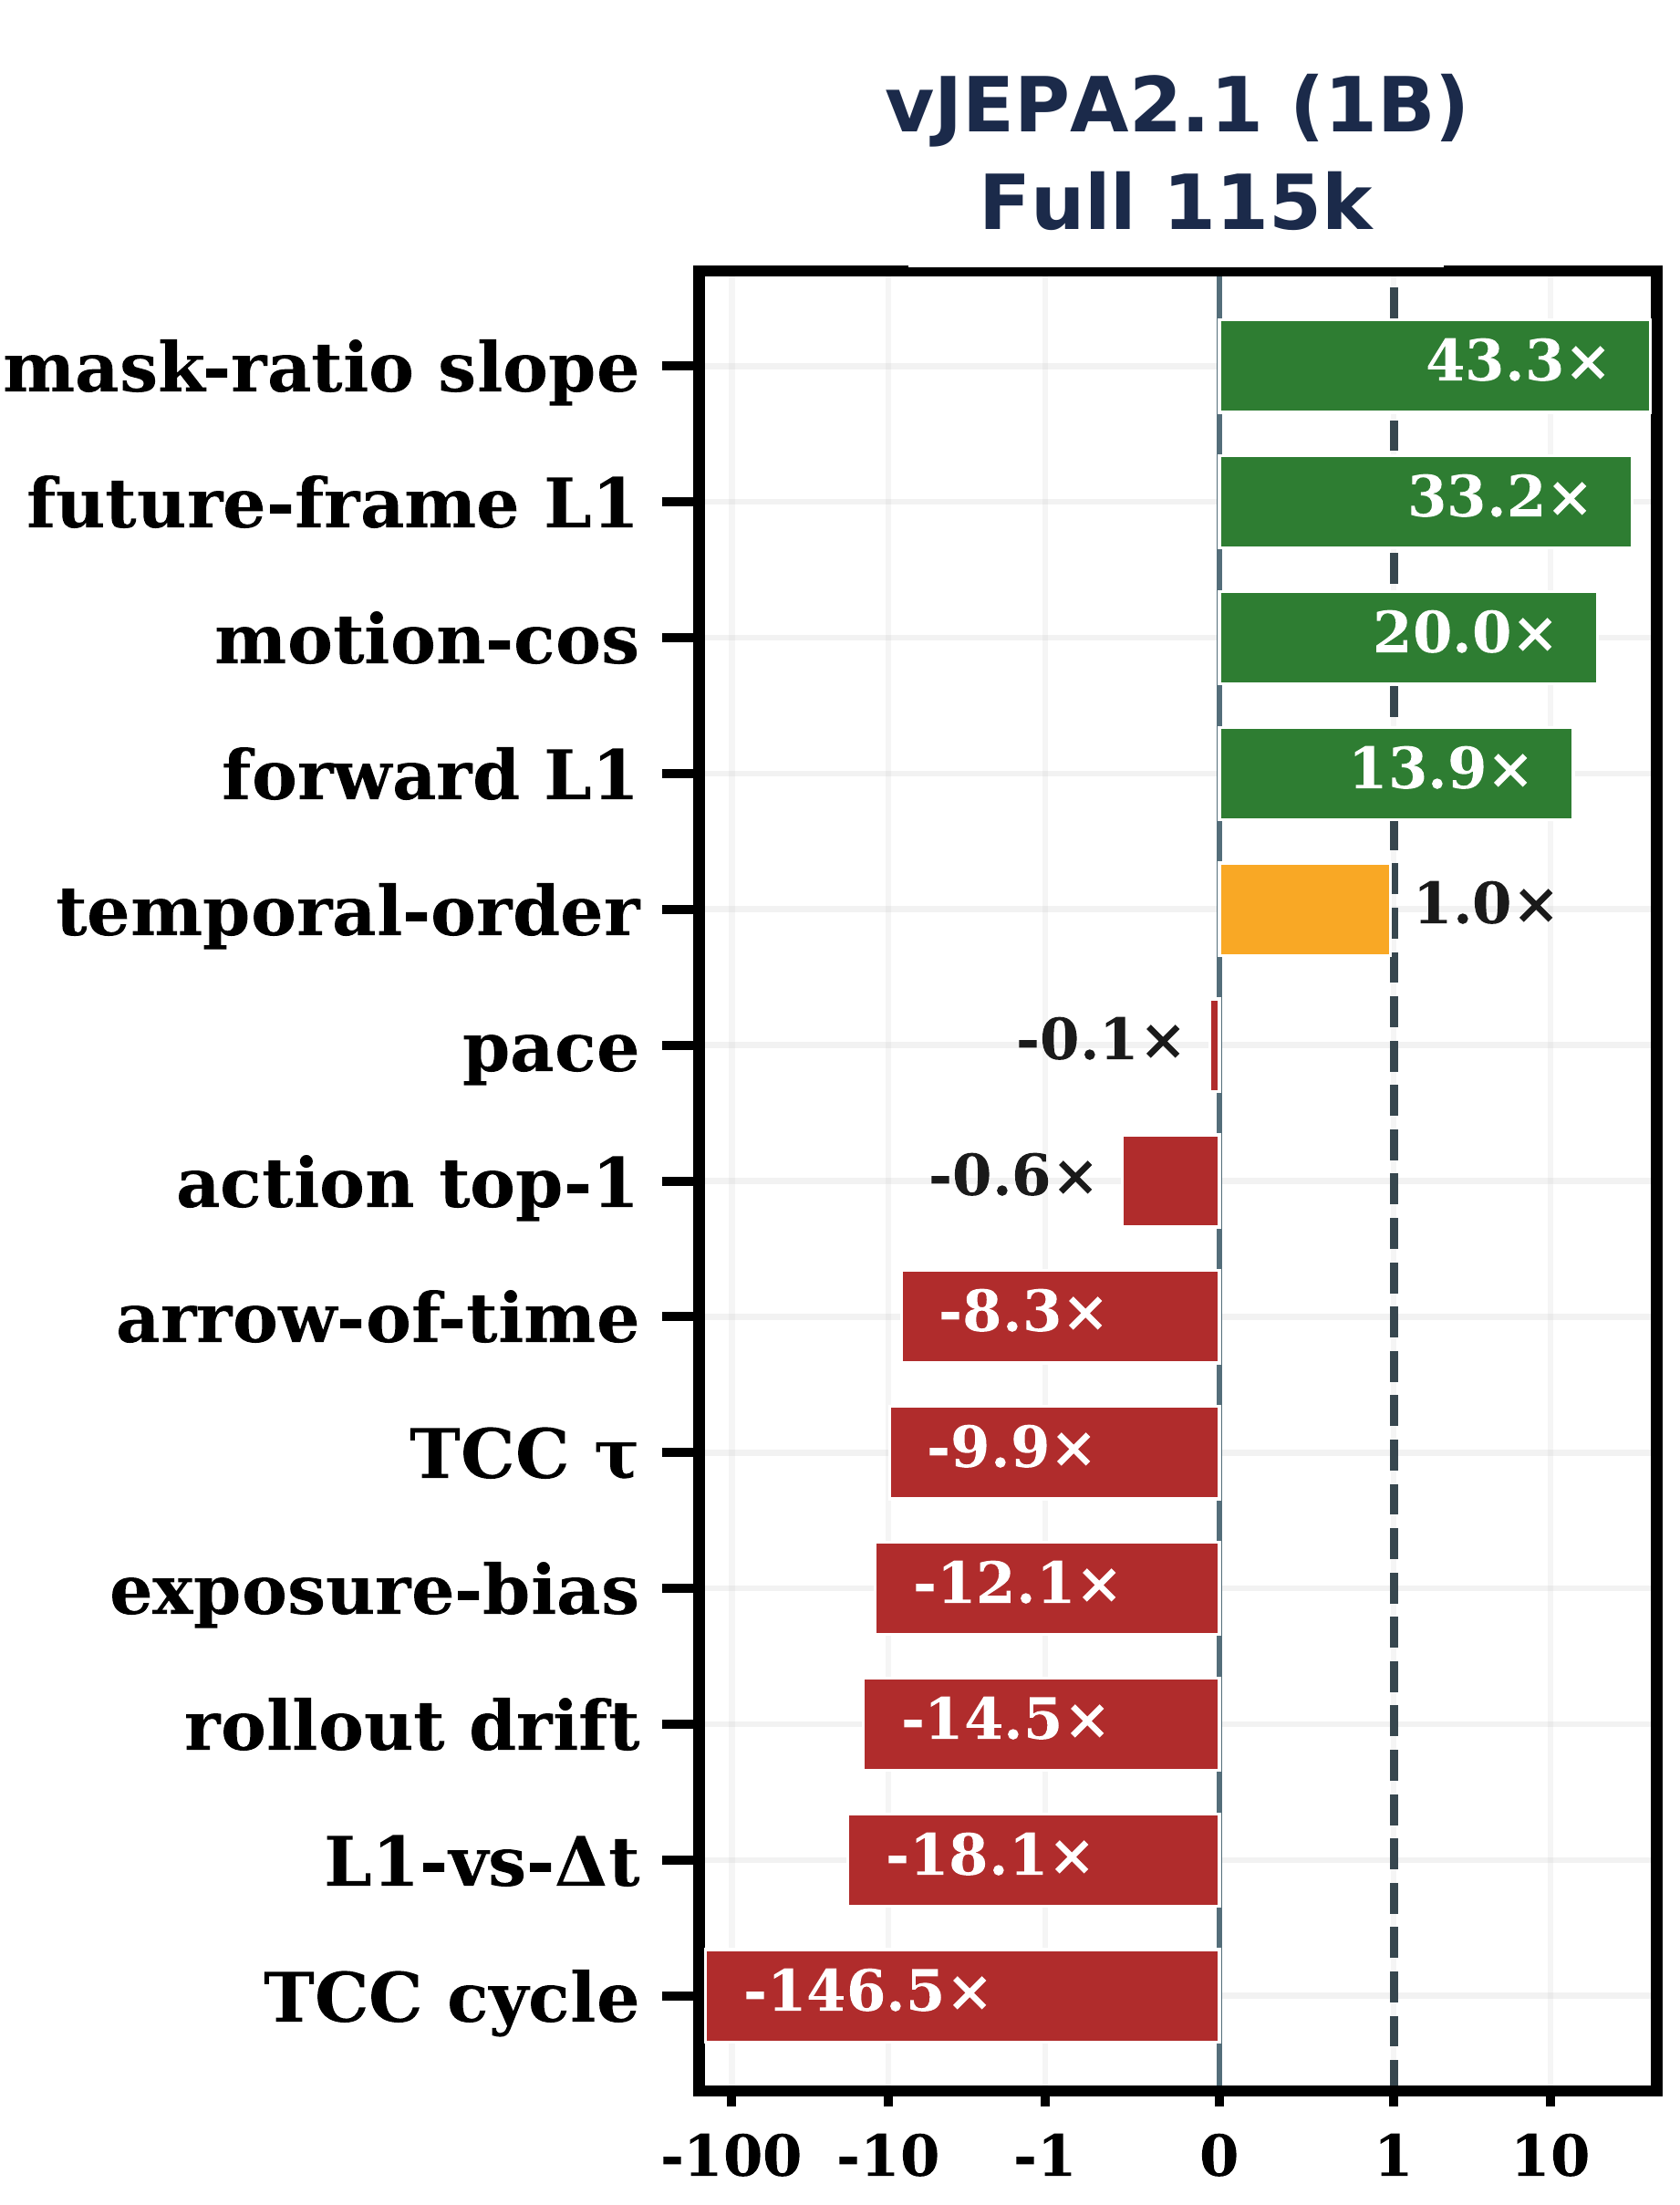
\includegraphics[width=0.97\columnwidth]{forest_115k_col.png}
\caption{Separation of the fixed FactorJEPA model from the strongest rival at 1B on the full corpus, in widths of the paired 95\% BCa interval (symmetric-log axis; dashed line: one width). Green: FactorJEPA ahead by at least one width; orange: ahead within the interval; red: the rival ahead.}
\label{fig:forest}
\end{figure}

\paragraph{Findings.}
With limited data (Table~\ref{tab:headline}), FactorJEPA separates from the best rival on Future-frame L1 and Forward L1 at both scales and on Mask-ratio slope at 1B, while Motion cosine favors full fine-tuning. After full 115k-clip training, against the two rivals trained at that scale (LoRA and the frozen backbone), FactorJEPA separates on all four diagnostics, Motion cosine included (Figure~\ref{fig:forest}), by 13.9 (Forward L1) to 43.3 (Mask-ratio slope) interval widths, a 2.7\% lower Future-frame L1 and a 19\% flatter Mask-ratio slope than LoRA. At 115k the Motion cosine lead is over LoRA and the frozen backbone; full fine-tuning, which leads on Motion cosine at 10k, was not trained at 115k. Method rankings on the four diagnostics replicate from the 2B to the 1B backbone (Spearman $\rho \geq 0.895$). The full-data evaluation also shows a trade-off in temporal coherence: below the rule, the best rival leads at 115k on six diagnostics (rollout drift, exposure bias, L1-versus-$\Delta t$ decay, arrow-of-time, and the two TCC measures) by 8.3 to 146.5 interval widths. FactorJEPA's strength is one-step prediction of crowded scenes, while the rivals keep the advantage on the coherence of long predicted futures.

\paragraph{Why the rivals lead on coherence.} The coherence diagnostics reward temporal cues learned from general video. Of the 23 cells in the lower nine rows of Table~\ref{tab:headline} that a rival wins, 13 go to the frozen backbone, which leads on arrow-of-time and both TCC measures in all three regimes, and 5 to plain continued pretraining, the starting point of every other trained method. Adapting to the corpus at all costs some of these cues: continued pretraining already lowers arrow-of-time accuracy at 2B from 0.965 to 0.952. On the 10k test clips at 2B, the staged schedule on raw clips costs more (arrow-of-time 0.935; exposure bias from 0.038 to 0.045), and the curriculum's clips recover part of the TCC loss (Kendall $\tau$ from 0.252 to 0.274) while raising exposure bias to 0.048; the 95\% intervals before and after each of these steps do not overlap. At 1B the staged schedule shows no such cost (exposure bias 0.037, 0.035, and 0.034 for plain, RAW, and Ours).

\begin{table}[t]
\centering
\small
\setlength{\tabcolsep}{3pt}
\begin{tabular}{llrrrr}
\toprule
 & Adaptation & Fut.\ L1$\downarrow$ & Fwd.\ L1$\downarrow$ & Mask$\downarrow$ & Motion$\uparrow$ \\
\midrule
2B & plain & 0.533 & 0.558 & 0.0625 & \textbf{0.151} \\
 & RAW & 0.497 & \textbf{0.528} & 0.0565 & 0.133 \\
 & Ours & \textbf{0.496} & 0.529 & \textbf{0.0531} & 0.116 \\
\midrule
1B & plain & 0.607 & 0.628 & 0.0586 & 0.054 \\
 & RAW & \textbf{0.587} & \textbf{0.611} & 0.0528 & \textbf{0.060} \\
 & Ours & 0.590 & 0.614 & \textbf{0.0515} & 0.048 \\
\bottomrule
\end{tabular}
\caption{Where the gain comes from, 10k clips, 1,825 test clips. Plain: continued pretraining, the starting point of both other rows. RAW: the same staged adaptation as Ours on raw clips only. Ours: the staged adaptation on the curriculum's layout, agent, and interaction clips. Every RAW-minus-plain and Ours-minus-RAW difference excludes zero at 95\% under both clip and source-video resampling (127 videos), except the Ours-minus-RAW difference in Future-frame L1 at 2B.}
\label{tab:ladder}
\end{table}

\paragraph{Where the gain comes from.} Table~\ref{tab:ladder} separates two contributions. The staged adaptation is the main source of the predictive gain: on raw clips alone it lowers Future-frame L1 by 0.036 (2B) and 0.020 (1B) below plain continued pretraining, and it already beats LoRA on Future-frame and Forward L1 at both scales. The automatically built layout, agent, and interaction clips add a specific property, robustness to missing evidence: they flatten the Mask-ratio slope by \nLadderMaskTwoB{} at 2B and \nLadderMaskOneB{} at 1B, so prediction degrades more slowly as more of the scene is masked. Masking is a controlled proxy for road users hidden by others, not a test on real occlusion. In exchange the clips lower Motion cosine at both scales and raise Forward L1 by 0.001 at 2B and Future-frame and Forward L1 by about 0.003 at 1B. On \nHeldoutClips{} clips from \nHeldoutVideos{} videos unused in training, the 1B rows keep every sign and the lead over LoRA holds except on Motion cosine (video-level intervals).


\section{What This Offers Mobility Agents}

A vehicle or robot moving among pedestrians and mixed traffic has to anticipate road users it can only partly see. Our results support that use in part. One-step prediction of crowded scenes improves at every scale and data size tested, and the layout, agent, and interaction clips make the model degrade more slowly as more of the scene is hidden, which is the situation of occluded road users. Temporal coherence over longer rollouts, which matters for planning several seconds ahead, is where the rivals still lead. At inference the model needs only monocular video, with no detector, HD map, or LiDAR, which matters in the many cities where such maps do not exist and road users rarely follow lanes. DENSEWORLD-115k also gives a benchmark for this regime that is not tied to driving metrics, which we hope the workshop community will extend with interaction-level labels.

\section{Scope and Next Steps}
\label{sec:scope}

The evaluation characterizes predictive representations: every diagnostic is measured in the frozen V-JEPA embedding space or with a small probe trained on it, and the interaction clips are candidates chosen by a proximity and relative-motion rule. Trajectory forecasting, a comparison with a calibrated social-force or agent-based model, and a check of the candidates against human judgements of who yields to whom lie outside the reported evaluation and are the next tests. The main protocol holds out clips (a video-disjoint check at 1B agrees, Section~4), and no city is held out. The results cover Indian footage and one training run per configuration; city-level and wider video-level splits, other dense-traffic regions, and repeated runs are the natural extensions.


{\small
\bibliography{../common/factorjepa}
}

\end{document}
